\documentclass[tikz,border=2pt,11pt]{standalone}
\usetikzlibrary{positioning}
\usetikzlibrary{arrows.meta}
\usetikzlibrary{calc}
\usetikzlibrary{decorations.markings}
\usetikzlibrary{fit}
\usepackage{amsmath}
\usepackage{amssymb}
\usepackage{mathrsfs}
\usepackage{bm}
\usepackage{graphicx}
\usepackage{tikz}
\renewcommand{\bibsection}{\section*{\refname}\addcontentsline{toc}{section}{\refname}}
\newcommand{\kk}{k}
\newcommand{\Fp}{\mathbb F_p}
\newcommand{\Zp}{\mathbb Z_p}
\newcommand{\Qp}{\mathbb Q_p}
\newcommand{\Cp}{\mathbb C_p}
\newcommand{\Cflat}{C^\flat}
\newcommand{\C}{\mathbb C}
\newcommand{\Z}{\mathbb Z}
\newcommand{\Q}{\mathbb Q}
\newcommand{\R}{\mathbb R}
\newcommand{\N}{\mathbb N}
\newcommand{\cO}{\mathcal O}
\newcommand{\cF}{\mathcal F}
\newcommand{\cL}{\mathcal L}
\newcommand{\cts}{\mathrm{cts}}
\newcommand{\ctensor}{\widehat{\otimes}}
\newcommand{\RGamma}{\mathbf R\Gamma}
\newcommand{\RHom}{\mathbf R\operatorname{Hom}}
\newcommand{\Rlim}{\mathop{\mathbf R\!\varprojlim}}
\DeclareMathOperator*{\colim}{colim}
\DeclareMathOperator{\id}{id}
\DeclareMathOperator{\Fr}{Fr}
\DeclareMathOperator{\Cartier}{C}
\DeclareMathOperator{\Hom}{Hom}
\DeclareMathOperator{\End}{End}
\DeclareMathOperator{\Ext}{Ext}
\DeclareMathOperator{\Tor}{Tor}
\DeclareMathOperator{\Spec}{Spec}
\DeclareMathOperator{\Spf}{Spf}
\DeclareMathOperator{\Spa}{Spa}
\DeclareMathOperator{\GL}{GL}
\DeclareMathOperator{\Gal}{Gal}
\DeclareMathOperator{\Aut}{Aut}
\DeclareMathOperator{\Lie}{Lie}
\DeclareMathOperator{\Ind}{Ind}
\DeclareMathOperator{\Coind}{Coind}
\DeclareMathOperator{\Res}{Res}
\DeclareMathOperator{\Pro}{Pro}
\DeclareMathOperator{\Perf}{Perf}
\DeclareMathOperator{\coker}{coker}
\DeclareMathOperator{\im}{im}
\DeclareMathOperator{\rk}{rk}
\DeclareMathOperator{\rank}{rank}
\DeclareMathOperator{\tr}{tr}
\DeclareMathOperator{\Tr}{Tr}
\DeclareMathOperator{\res}{res}
\DeclareMathOperator{\supp}{supp}
\DeclareMathOperator{\ord}{ord}
\DeclareMathOperator{\length}{length}
\DeclareMathOperator{\ad}{ad}
\begin{document}
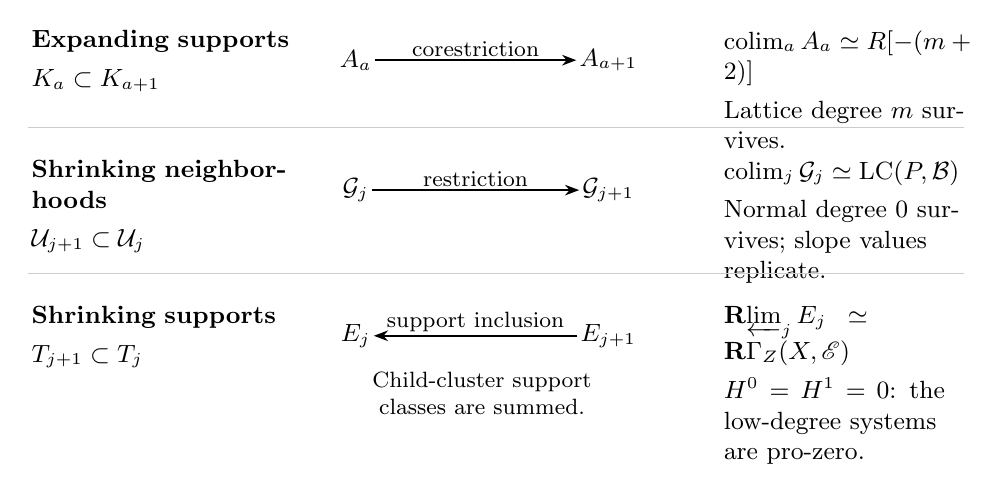
\begin{tikzpicture}[
  x=.98\linewidth,y=1cm,
  every node/.style={font=\small,inner sep=1pt},
  heading/.style={anchor=north west,align=left,text width=.28\linewidth},
  outcome/.style={anchor=north west,align=left,text width=.26\linewidth},
  transition/.style={-{Stealth[length=1.8mm]},semithick}
]
\node[heading] at (0,0)
  {\textbf{Expanding supports}\\[3pt]
   $K_a\subset K_{a+1}$};
\node (a0) at (.35,-.42) {$A_a$};
\node (a1) at (.62,-.42) {$A_{a+1}$};
\draw[transition] (a0) -- node[above,font=\footnotesize]
  {corestriction} (a1);
\node[outcome] at (.74,0)
  {$\colim_a A_a\simeq R[-(m+2)]$\\[3pt]
   Lattice degree $m$ survives.};
\draw[black!20] (0,-1.28) -- (1,-1.28);

\node[heading] at (0,-1.65)
  {\textbf{Shrinking neighborhoods}\\[3pt]
   $\mathcal U_{j+1}\subset\mathcal U_j$};
\node (g0) at (.35,-2.07) {$\mathcal G_j$};
\node (g1) at (.62,-2.07) {$\mathcal G_{j+1}$};
\draw[transition] (g0) -- node[above,font=\footnotesize]
  {restriction} (g1);
\node[outcome] at (.74,-1.65)
  {$\colim_j\mathcal G_j\simeq\operatorname{LC}(P,\mathcal B)$\\[3pt]
   Normal degree $0$ survives; slope values replicate.};
\draw[black!20] (0,-3.13) -- (1,-3.13);

\node[heading] at (0,-3.5)
  {\textbf{Shrinking supports}\\[3pt]
   $T_{j+1}\subset T_j$};
\node (e0) at (.35,-3.92) {$E_j$};
\node (e1) at (.62,-3.92) {$E_{j+1}$};
\draw[transition] (e1) -- node[above,font=\footnotesize]
  {support inclusion} (e0);
\node[outcome] at (.74,-3.5)
  {$\Rlim_j E_j\simeq\RGamma_Z(X,\mathscr E)$\\[3pt]
   $H^0=H^1=0$: the low-degree systems are pro-zero.};
\node[align=center,font=\footnotesize,text width=.40\linewidth]
  at (.485,-4.65) {Child-cluster support classes are summed.};
\end{tikzpicture}
\end{document}
